\documentclass[a4paper]{proc}
\title{Fitting SARMA Models Onto Activity and Skin Temperature Time Series Data}
\author{Sherman Ip$\qquad$March 10, 2016}

\usepackage{amsmath}
\usepackage{amsfonts}
\usepackage{amssymb}
\usepackage{graphicx}
\usepackage{subcaption}
\usepackage{caption}

\DeclareMathOperator{\expectation}{E}

\newcommand{\euler}{\mathrm{e}}
\newcommand{\diff}{\mathrm{d}}
\newcommand{\T}{^\textup{T}}
\newcommand{\vect}[1]{\mathbf{#1}}
\newcommand{\vectGreek}[1]{\boldsymbol{#1}}
\newcommand{\matr}[1]{\mathsf{#1}}
\newcommand{\dotdotdot}{\vphantom{.}_{\cdots}}
\newcommand{\backshift}{\widehat{B}}

\begin{document}

\maketitle

\begin{abstract}
Seasonal autoregressive moving average (SARMA) models were fitted onto time series data on activity and skin temperature of 4 subjects. The number of SARMA parameters were selected using information criterions. It was found the SARMA model did not fit well with the activity time series because the forecast error were too big to be of practical use. For the temperature time series, seasonal autoregressive parameters were favoured.
\end{abstract}

\section{Introduction}
Suppose a time series $\{Y_1,Y_2,\dotdotdot,Y_T\}$ was observed and, without lost of generality, has zero mean. An ARMA$(p,q)$ model can be fitted which has the form
\begin{equation}
Y_t = \sum_{i=1}^{p} \phi_i Y_{t-i} + \epsilon_t - \sum_{j=1}^{q} \theta_{j} \epsilon_{t-j}
\label{eq:ARMA}
\end{equation}
where $\epsilon_t$ are some i.i.d.~distributed noise with zero mean and variance $\sigma^2$.

By using the backshift operator $\backshift$ where
\begin{align}
\backshift^k Y_t &= Y_{t-k} \\
\backshift^k \epsilon_t &= \epsilon_{t-k} \ ,
\end{align}
Equation \eqref{eq:ARMA} can be expressed as
\begin{equation}
Y_t = \sum_{i=1}^{p} \phi_i \backshift^i Y_{t} + \epsilon_t - \sum_{j=1}^{q} \theta_{j} \backshift^j \epsilon_{t}
\end{equation}
which can be rearranged to
\begin{equation}
\theta\left(\backshift\right)Y_t=\phi\left(\backshift\right)\epsilon_t
\end{equation}
where
\begin{align}
\phi(x)&=1-\sum_{i=1}^{p} \phi_i x \\
\theta(x)&=1-\sum_{i=1}^{q} \theta_i x
\end{align}
are called the AR and MA characteristic equations respectively.

Seasonality, of lag $s$, can be considered by including the AR and MA seasonal characteristic equations, $\Phi(x)$ and $\Theta(x)$ respectively, where
\begin{align}
\Phi(x) &= 1 - \sum_{i=1}^P \Phi_i x^{is} \\
\Theta(x) &= 1 - \sum_{j=1}^Q \Theta_j x^{js} \ .
\end{align}
The SARMA$(p,q)\times(P,Q)_s$ model uses the seasonal characteristic equation where the model has the form
\begin{equation}
\phi\left(\backshift\right)\Phi\left(\backshift\right)Y_t
=
\theta\left(\backshift\right)\Theta\left(\backshift\right)\epsilon_t
\end{equation}

Assuming the noise is Normally distributed, the maximum likelihood can be used to estimate the SARMA parameters: $\phi_1,\dotdotdot,\phi_p,\theta_1,\dotdotdot,\theta_q,\Phi_1,\dotdotdot\Phi_P,\Theta_1,\dotdotdot,\Theta_Q$. The assumption of Normal i.i.d.~noise can be checked by investigating the residuals of fitting the SARMA model onto the data.

The objective was to fit SARMA onto activity and skin temperature time series data and see how they perform.

\section{Methods}
Selecting $p,q,P,Q,s$ to use to fit the SARMA model, onto the time series, is troublesome because it involves investigating 5 parameters.

$s$ was selected and fixed to be 24 hours because it was observed, by inspection, that there may be a cyclic behaviour, with a period of 24 hours, in the time series.

The Akaike information criterion (AIC) and Bayesian information criterion (BIC) was used to select which $p,q,P,Q$ to use to fit the SARMA model onto the data. The information criterions have the form
\begin{align}
\textup{AIC}&=T\ln{\widehat{\sigma}^2}+(p+q+P+Q)2\\
\textup{BIC}&=T\ln{\widehat{\sigma}^2}+(p+q+P+Q)\ln{T}
\end{align}
where $\widehat{\sigma}^2$ is the estimated variance of the residuals. Firstly, ARMA$(p,q)$ models were fitted for $p=0,1,\dotdotdot,5$ and $q=0,1,\dotdotdot,5$. The $p,q$ pair which minimises an information criterion was selected and fixed. Secondly, SARMA$(p,q)\times(P,Q)_s$ models were fitted for $P=0,1,2$ and $Q=0,1,2$. The $P,Q$ pair was selected which minimises an information criterion. MATLAB \emph{regARMA} was used to fit the SARMA model onto the data.

The model was tested by fitting the SARMA model, using the AIC/BIC procedure, onto the first 3 days of the data. The model was then extrapolated to do a 24 hour forecast. Such a forecast was then compared with the actual data using the mean squared error (and the logarithmic scoring). That is suppose $\{\widehat{Y}_{T+1},\widehat{Y}_{T+2},\dotdotdot,\widehat{Y}_{T+h}\}$ was the forecast of $\{{Y}_{T+1},{Y}_{T+2},\dotdotdot,{Y}_{T+h}\}$, then the mean squared error (MSE) was calculated using
\begin{equation}
\textup{MSE} = \frac{\sum_{k=1}^{h}\left(\widehat{Y}_{T+k}-Y_{T+k}\right)^2}{h} \ .
\end{equation}

The forecast error, $\{\widehat{e}_{T+1},\widehat{e}_{T+2},\dotdotdot,\widehat{e}_{T+h}\}$, was obtained and used to estimate approximately the error in the MSE using the Delta method given as
\begin{equation}
\sigma_{\textup{MSE}} = \frac{2}{h}\sqrt{\sum_{k=1}^{h}\left(\widehat{Y}_{T+k}-Y_{T+k}\right)^2\left(\widehat{e}_{T+k}\right)^2} \ .
\end{equation}

\section{Results}
SARMA$(p,q)\times(P,Q)_{24}$ models were fitted onto the 8 time series data independently. As an example, Figure \ref{fig:sarmafit} shows the selected SARMA model, using AIC, being fitted onto the first 3 days of the time series of subject 8. The model was then extrapolated to do a 24 hour forecast.

It was observed that the forecast error on the activity time series blew up in the order of $\sim 10^2$. A forecast with such an error is practically useless thus it was considered that the SARMA model did not fit well with the activity time series.

The forecast error on the temperature time series was sensible and the mean squared errors along with the selected SARMA model is shown in Tables \ref{table:temp_AIC} and \ref{table:temp_BIC}. Comparing the two tables, the BIC consistently selected the SARMA model with less parameters, compared with AIC.

There was not much difference in the mean squared errors between using AIC or BIC to select the favourable SARMA model, even though the values of $p$ and $q$ did varied. In additional both information criterions favoured at least one 24 hour seasonal autoregressive parameter, thus it could be possible the seasonal part of the SARMA captures most of the behaviour of the time series.

\begin{table}[p]
\begin{center}
\begin{tabular}{ cccccc } 
 Data & p & q & P & Q & MSE ($\textup{g}^2$)\\
  \hline
 RA2 & 5 & 5 & 1 & 0 & $\sim10^2$\\
 RA8 & 2 & 4 & 2 & 0 & $\sim10^2$\\
 RA24& 4 & 5 & 0 & 0 & $\sim10^2$\\
 RA26& 4 & 4 & 2 & 0 & $\sim10^3$\\
\end{tabular}
\end{center}
\caption{The selected SARMA$(p,q)\times(P,Q)_{24}$ model, using AIC, to fit the first 3 days of activity time series. The 24 hour forecast was then assessed using the mean squared error.}
\label{table:ra_AIC}
\end{table}

\begin{table}[p]
\begin{center}
\begin{tabular}{ cccccc } 
 Data & p & q & P & Q & MSE ($\textup{g}^2$)\\
  \hline
 RA2 & 2 & 2 & 1 & 1 & $\sim10^2$\\
 RA8 & 1 & 0 & 2 & 0 & $\sim10^2$\\
 RA24& 3 & 2 & 2 & 0 & $\sim10^3$\\
 RA26& 1 & 0 & 1 & 1 & $\sim10^3$\\
\end{tabular}
\end{center}
\caption{The selected SARMA$(p,q)\times(P,Q)_{24}$ model, using BIC, to fit the first 3 days of activity time series. The 24 hour forecast was then assessed using the mean squared error.}
\label{table:ra_BIC}
\end{table}

\begin{table}[p]
\begin{center}
\begin{tabular}{ cccccc } 
 Data & p & q & P & Q & MSE ($^{\circ}\textup{C}^2$)\\
  \hline
 Temp2 & 2 & 4 & 2 & 0 & $1.71\pm0.09$\\
 Temp8 & 2 & 1 & 2 & 0 & $1.4\pm0.1$\\
 Temp24& 4 & 4 & 1 & 1 & $0.43\pm0.04$\\
 Temp26& 5 & 2 & 2 & 0 & $0.7\pm0.1$\\
\end{tabular}
\end{center}
\caption{The selected SARMA$(p,q)\times(P,Q)_{24}$ model, using AIC, to fit the first 3 days of temperature time series. The 24 hour forecast was then assessed using the mean squared error.}
\label{table:temp_AIC}
\end{table}

\begin{table}[p]
\begin{center}
\begin{tabular}{ cccccc } 
 Data & p & q & P & Q & MSE ($^{\circ}\textup{C}^2$)\\
  \hline
 Temp2 & 0 & 2 & 2 & 0 & $1.72\pm0.08$\\
 Temp8 & 2 & 1 & 2 & 0 & $1.4\pm0.1$\\
 Temp24& 2 & 4 & 1 & 1 & $0.36\pm0.03$\\
 Temp26& 2 & 0 & 2 & 0 & $0.69\pm0.06$\\
\end{tabular}
\end{center}
\caption{The selected SARMA$(p,q)\times(P,Q)_{24}$ model, using BIC, to fit the first 3 days of temperature time series. The 24 hour forecast was then assessed using the mean squared error.}
\label{table:temp_BIC}
\end{table}

\begin{figure*}[p]
    \begin{subfigure}[b]{\textwidth}
        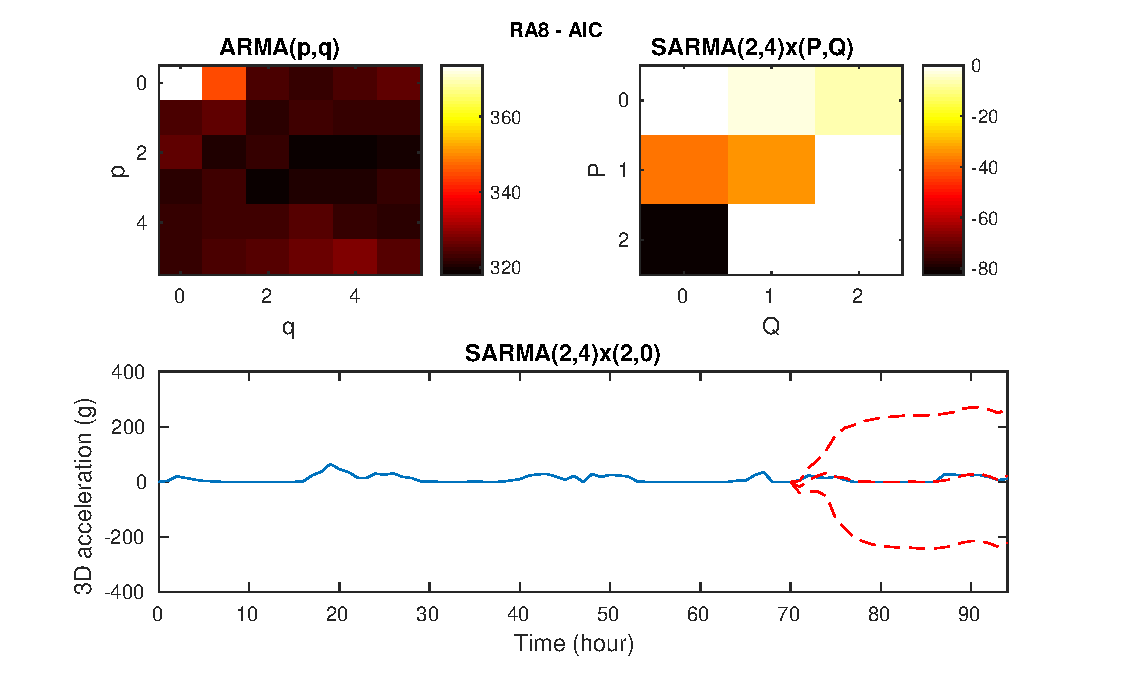
\includegraphics[width=\textwidth]{aic_ra_8.eps}
        \caption{Activity Time Series}
    \end{subfigure}
    \begin{subfigure}[b]{\textwidth}
        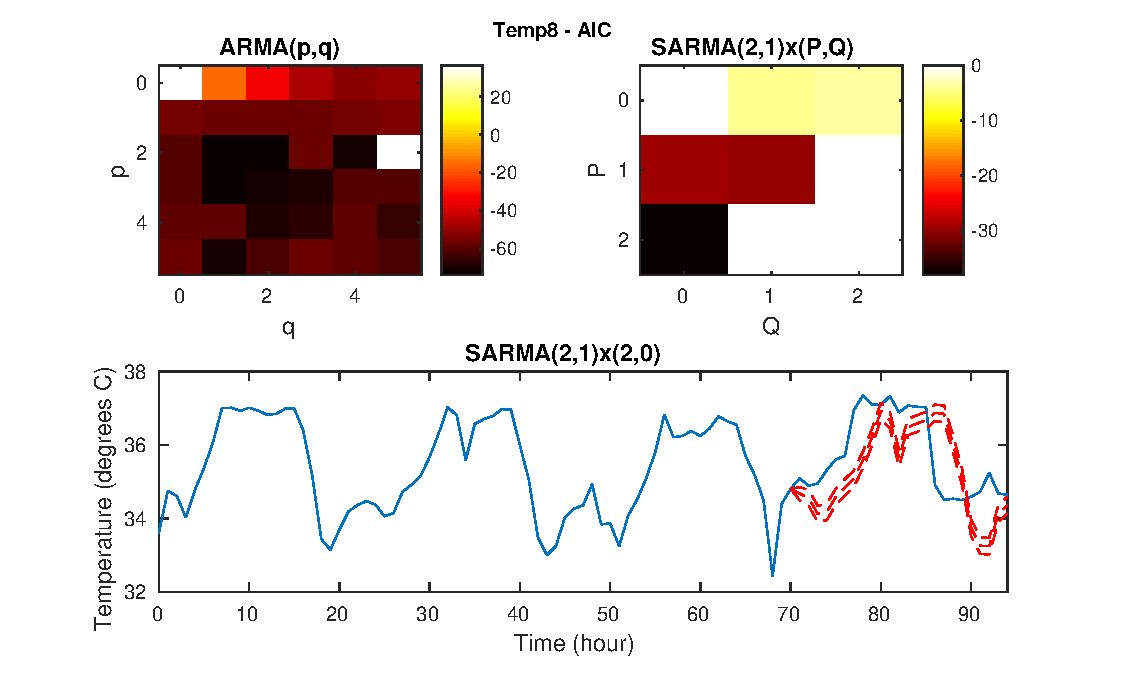
\includegraphics[width=\textwidth]{aic_temp_8.eps}
        \caption{Skin Temperature Time Series}
    \end{subfigure}
    \caption{Top-left: AIC fitting ARMA$(p,q)$ onto the first 3 days of the time series. Top-right: Difference in AIC when fitting SARMA(2,1)$\times(P,Q)_{24}$ compared with ARMA(2,1). Bottom: SARMA(2,1)$\times(2,0)_{24}$ was fitted and then extrapolated to do a 24 hour forecast with an error (red dotted lines). This was compared with the actual time series (solid blue line).}
    \label{fig:sarmafit}
\end{figure*}

\section{Conclusion}
The SARMA model did not fit well with the activity time series because the forecast error were unacceptably large. Such a bad fit could be because of how the time series is bounded at zero or above. One possible fix is to do some sort of logarithmic transform on the time series.

For the temperature time series, it was found seasonal autoregressive lags was favoured all the time using either the AIC or BIC.

The fit could be better if the time series was longer than 4 days.

\end{document}
